%% sudo yum install tetex
%% sudo yum install texlive-elsarticle.noarch  texlive-sttools.noarch texlive-lipsum.noarch
%% pdflatex neural_network.tex && bibtex neural_network.aux && pdflatex neural_network.tex && pdflatex neural_network.tex


%\documentclass[a4paper,12pt]{}
\documentclass[final, paper=letter,5p,times,twocolumn]{elsarticle}
%\documentclass[preprint,review,8pt,times]{elsarticle}


%% or use the graphicx package for more complicated commands
%\usepackage{changebar}
\usepackage{graphicx}
\usepackage{caption}
\usepackage{subcaption}
\usepackage{multirow}
%% or use the epsfig package if you prefer to use the old commands
%% \usepackage{epsfig}

%% The amssymb package provides various useful mathematical symbols
\usepackage{tikz}
\usepackage{amsmath,amsfonts,amsthm,multicol,bm,lipsum} % Math packages
\usepackage{cuted}
%\usepackage{dsfont} % mathds{1}
%\usepackage{widetext} % 
\usepackage{listings}
\usepackage{amssymb}
\usepackage{hyperref}
%
%\usepackage[]{algorithm2e}
%% Macro
\newcommand{\ToDo}[1]{ToDo: \textbf{\textit{#1}}}
\newcommand{\CA}{computational anatomy}
%
\newdefinition{definition}{Definition}%
\newtheorem{theorem}{Theorem}%
\newtheorem{corollary}{Corollary}[theorem]
\newtheorem{lemma}[theorem]{Lemma}
%\newproposition{proposition}{Proposition}%
%\newlemma{lemma}{Lemma}%
%\AtEndEnvironment{theorem}{\null\hfill\qedsymbol}%

\begin{document}
%%%%%%%%%%%%%%%%%%%%%%%%%%%%%%%%%%%%%%%%%%%%%%%%%%%%%%%%%%%%%%%%%%%%%%%%%%
%%%%%%%%%%%%%%%%%%%%%%%%%%%%%%%%%%%%%%%%%%%%%%%%%%%%%%%%%%%%%%%%%%%%%%%%%%
%%%%%%%%%%%%%%%%%%%%%%%%%%%%%%%%%%%%%%%%%%%%%%%%%%%%%%%%%%%%%%%%%%%%%%%%%%
%%%%%%%%%%%%%%%%%%%%%%%%%%%%%%%%%%%%%%%%%%%%%%%%%%%%%%%%%%%%%%%%%%%%%%%%%%
\begin{frontmatter}

\title{Neural network}

\author[label1]{Yann Cobigo\corref{cor1}}
\address[label1]{University of California, San Francisco | ucsf.edu}
%\address[label2]{Address Two\fnref{label4}}

%\cortext[cor1]{I am corresponding author}
%\fntext[label3]{I also want to inform about\ldots}
%\fntext[label4]{Small city}

\ead{yann.cobigo@ucsf.edu}
\ead[url]{https://github.com/YannCobigo}

%% \author[label5]{Author Two}
%% \address[label5]{Some University}
%% \ead{author.two@mail.com}
%% 
%% \author[label1,label5]{Author Three}
%% \ead{author.three@mail.com}

\begin{abstract}
 \lipsum[11-15]
\end{abstract}

\begin{keyword}
%% keywords here, in the form: keyword \sep keyword
Fijee \sep electrode \sep PEM \sep CEM
%% MSC codes here, in the form: \MSC code \sep code
%% or \MSC[2008] code \sep code (2000 is the default)
\end{keyword}

\end{frontmatter}

%%%%%%%%%%%%%%%%%%%%%%%%%%%%%%%%%%%%%%%%%%%%%%%%%%%%%%%%%%%%%%%%%%%%%%%%%%
%%%%%%%%%%%%%%%%%%%%%%%%%%%%%%%%%%%%%%%%%%%%%%%%%%%%%%%%%%%%%%%%%%%%%%%%%%
%%%%%%%%%%%%%%%%%%%%%%%%%%%%%%%%%%%%%%%%%%%%%%%%%%%%%%%%%%%%%%%%%%%%%%%%%%
%%%%%%%%%%%%%%%%%%%%%%%%%%%%%%%%%%%%%%%%%%%%%%%%%%%%%%%%%%%%%%%%%%%%%%%%%%

\section{Introduction}

\lipsum[100-104]

\paragraph{Perceptrons}{One of the key concept of the neural network is the perceptron algorithm. The perceptron was one of the first machine learning algorithm used with computers. It was introduce in neural network as multilyer perceptron (MLP). The pricipal of classification using perceptron seat on fitting linear model $\omega^{T}\alpha > \theta$, where $\omega$ is a vector of $N$ weights, $\alpha$ is a vector of $N$ predictors and $\theta$ is a threshold. We can incorporate the threshold in the dot product, $f(\alpha) = \omega^{T}\alpha - \theta \times 1 = \sum_{i=0}^{N} \omega_{i}\alpha_{i} > 0$, $\omega = (\omega_{0}, \omega_{0}, \dots, \omega_{N-1}, \theta)^{T}$ and $\alpha = (\alpha_{0}, \alpha_{1}, \dots, \alpha_{N-1}, 1)^{T}$.}

\paragraph{Inputs}{For the different type of neural networks we would like to accomplish, the input classes must be very differents. Most of the time we are going to work with medical images, implying using a dimensional correlation like the convolutional neural network (CNN). Unlike most of the machine learning algorithm taking vectors as input, CNN void the space decorrelation from the vectorization. However, providing different calsses for different inputs could offer some flexibility.}

\ToDo{check ll sort of input we would want.} \\

%%%%%%%%%%%%%%%%%%%%%%%%%%%%%%%%%%%%%%%%%%%%%%%%%%%%%%%%%%%%%%%%%%%%%%%%%%
%%%%%%%%%%%%%%%%%%%%%%%%%%%%%%%%%%%%%%%%%%%%%%%%%%%%%%%%%%%%%%%%%%%%%%%%%%
\section{Functions}

A neuron is represented with an activation $a_{l_{i}} = \sum_{l_{j} = 0}^{L_{j}} \omega_{l_{i}l_{j}} z_{l_{j}}$, integrating pulses from other neurons, and its activation function $z_{l_{i}} = f(a_{l_{i}})$, the firering process of the neuron. Usually, the activation function is taken non-linear. Following the litterature, we will mostly use $\tanh$ or logistic function.

\subsection{Activation functions}

Activation functions used for layers of neurons are the hyperbolic tangent, the logistic or the rectified linear unit (ReLU). Expcept for special layers like the last layer of a fully connected network. The derivetive of these funetion are:

\begin{itemize}
\item hyperbolic tangent: $f = \tanh \rightarrow f' = 1 - \tanh \times \tanh$,
\item logistic: $\sigma = \frac{1}{1+e^{-x}} \rightarrow \sigma' = \sigma (1 - \sigma)$,
\item ReLU: $x^{+} = \max(0,x) \rightarrow 1$ if $x^{+} = x$, 0 otherwise.
\end{itemize}
\ToDo{how to make the choise of the activation function.}

\subsubsection{Soft maximum}
\label{soft_max_sec}

The soft maximum is often used in classfication problem involving multiple output classes. the output can be interpretated as probability following the distribution:

\begin{equation}
  g(a_{l_{k}}) = \frac{e^{a_{l_{k}}}}{\mathcal{Z}}
  \label{soft_max}
\end{equation}

Where $\mathcal{Z}$ is the partition function normalizing the distribution. Derivating the soft maximum in function of the parameter $a_{k}$ gives us:

\begin{equation*}
  \begin{split}
    \frac{\partial g(a_{k})}{\partial a_{k'}} = & \left \lbrack \delta_{kk'} e^{a_{k'}} \mathcal{Z} - e^{a_{k'}}\frac{\partial \mathcal{Z}}{\partial a_{k'}} \right \rbrack \times \frac{1}{\mathcal{Z}^{2}}\\
    = & \left \lbrack \delta_{kk'} e^{a_{k'}} \mathcal{Z} - e^{a_{k'}} \sum_{k''} \delta_{kk''} e^{a_{k''}}  \right \rbrack \times \frac{1}{\mathcal{Z}^{2}}\\
    = & \frac{\delta_{kk'} e^{a_{k'}}}{\mathcal{Z}} - z_{k}z_{k'}\\
  \end{split}
\end{equation*}

\lipsum[2-2]

\subsection{Cost functions}

Training the neural network uses the gradient method. All functions representing the neural activity needs to be differentiable, including the cost fuction. \lipsum[3-3]

\subsubsection{Least-squarre cost function}

\begin{equation}
  E = \frac{1}{2} \sum_{i = 1}^{n} \| \bm{z}(\bm{x}_{i}) - \bm{t}_{i} \|^{2}
  \label{least_squarre}
\end{equation}

\subsubsection{Cross entropy cost function}
\label{Cross_entropy_cost_function_sec}

In information theory, the cross entropy between two probability distributions $p$ and $q$ over the same underlying set of events measures the average number of bits needed to identify an event drawn from the set, if a coding scheme is used that is optimized for an "unnatural" probability distribution $q$, rather than the "true" distribution $p$. In classification, the cross entropy for the distributions $t$, labels, and $z$, reconstructed solution, over a given set is defined as follows:

\begin{equation}
  E = - \sum_{i = 1}^{n}\sum_{l'_{k} = 1}^{L_{k}} t_{l'_{k}} \ln z_{l'_{k}} =  - \sum_{i = 1}^{n} E_{i}
  \label{cross_entropy}
\end{equation}

$t_{l'_{k}}$ represents the known label, $z_{l'_{k}} = y_{k}$ represents the response of the system, $n$ is the number of participents. 

In this section, we are going to derivate the cross entropy~(\ref{cross_entropy}). To simplify the equation, we are derivating the cost function only for one subject and omitte the subscript $i$. At the output layer, the activation is $a_{l_{k}} = \sum_{l_{k-1} = 0}^{L_{k-1}} \omega_{l_{k}l_{k-1}} z_{l_{k-1}}$. The derivative of the cost function in function of the activtion is called the {\it error} and is written:

\begin{equation}
  \delta_{k} = \frac{\partial E_{i}}{\partial a_{l_{k}}} = - \sum_{l'_{k} = 1}^{L_{k}} t_{l'_{k}} \times \frac{1}{z_{l'_{k}}} \frac{\partial z_{l'_{k}}}{\partial a_{k}}
  \label{cost_function_error}
\end{equation}

In the case of the last activation fuction for the output layer is a soft maximum, we can use the result of the soft maximum derivative from the paragraph~\ref{soft_max_sec}:

\begin{equation*}
  \begin{split}
    \delta_{k} = & - \sum_{l'_{k} = 1}^{L_{k}} t_{l'_{k}} \times \frac{1}{z_{l'_{k}}} \left \lbrack  \frac{\delta_{kk'} e^{a_{l'_{k}}}}{\mathcal{Z}} - z_{l'_{k}}z_{l_{k}} \right \rbrack \\
    = & - \sum_{l'_{k} = 1}^{L_{k}} t_{l'_{k}} \times \frac{1}{z_{l'_{k}}} \frac{\delta_{kk'} e^{a_{l'_{k}}}}{\mathcal{Z}} +  \sum_{l'_{k} = 1}^{L_{k}} t_{l'_{k}} z_{l_{k}} \\
    = & - t_{l_{k}} +  z_{k} \\
  \end{split}
\end{equation*}



Which is exactly the same result as we would get in the case of a least-square cost function. \lipsum[4-4]


%%%%%%%%%%%%%%%%%%%%%%%%%%%%%%%%%%%%%%%%%%%%%%%%%%%%%%%%%%%%%%%%%%%%%%%%%%
%%%%%%%%%%%%%%%%%%%%%%%%%%%%%%%%%%%%%%%%%%%%%%%%%%%%%%%%%%%%%%%%%%%%%%%%%%
\section{Convolutional neural network}

Convolutional neural networks (CNNs) are a biologically-inspired variation of the MLPs. Neurons in CNNs share weights unlike in MLPs where each neuron has a separate weight vector. This sharing of weights ends up reducing the overall number of trainable weights hence introducing sparsity. The output image is downsampled to reduce the number of weights for the next neural network and prevent overfitting.

\subsection{Description and notation}

CNNs consists of convolutional layers which are characterized by an input map $Im$, a bank of filters $Ker$ with biases $b$ per layer. Utilizing the weights sharing strategy, each neuron in the feature map is the result of the convolution of a kernel with a region in the input image, called the {\it local receptive field for the hidden neuron}, Fig.~\ref{fig:Convolutional_layers}. The local receptive field is a three dimensions window on the input voxels. This is then followed by a pooling operation which is a form of down-sampling of the newly produced feature map. Existing between the convolution and the pooling layer is an activation function such as the Rectified Linear unit ({\it ReLu}) layer; a non-saturating activation is applied element-wise, {\it i.e.} $f(x) = \max(0,x)$ thresholding at zero. After several convolutional and pooling layers, the image size (feature map size) is reduced and more complex features are extracted. \\

\begin{figure}[htbp]
   \begin{center}
      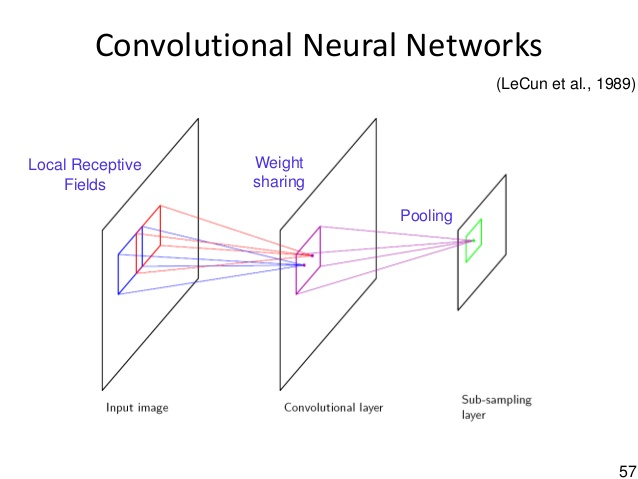
\includegraphics[scale=0.3, angle=0]{images/Bishop_cnn_layer.jpg}
   \end{center}
   \caption{Convolutional layers. Receptive field of a convolutional layer. Each neuron of the feature map is the result of the convolution of a kernel with the input image in the receptive field.}
  \label{fig:Convolutional_layers} 
\end{figure}

\begin{figure*}[htbp]
   \begin{center}
      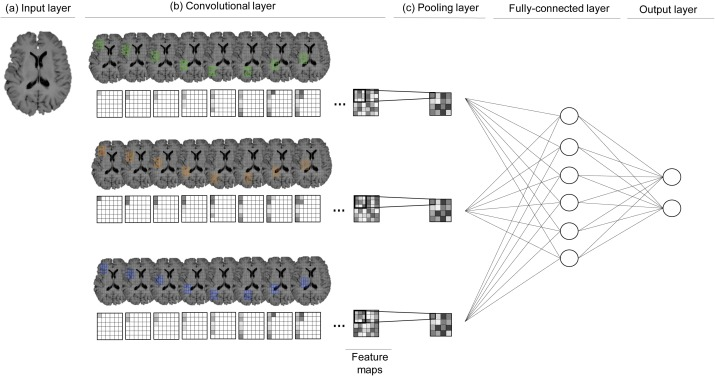
\includegraphics[scale=1., angle=0]{images/1-s2_0-S0149763416305176-gr4.jpg}
   \end{center}
   \caption{Generic structure of a CNN. For illustrative purpose, this example only has one layer of each type; a real-world CNN, however, would have several convolutional and pooling layers (usually interpolated) and one fully-connected layer. (a) Input layer. In its simplest way, the data is inputted into the network in such a way that each pixel corresponds to one node in the input layer. (b) Convolutional layer. A $3 \times 3$ filter or kernel (in green) is used to multiply the spatially corresponding $3 \times 3$ nodes in the image. The resulting weighted sum is then passed through a nonlinear function to derive the output value of one node in the feature map. The repetition of this same operation across all possible receptive fields results in one complete feature map. The same procedure with different kernels (in orange and blue) will result in separate complete feature maps. (c) Pooling layer. The size of each feature map can be reduced by taking the maximum value (or average) from a receptive field in the previous layer. (For interpretation of the references to colour in this figure legend, the reader is referred to the web version of this article.)}
  \label{fig:features_maps} 
\end{figure*}

\paragraph{Feature map}{The weights sharing strategy means that all the neurons in the first hidden layer detect exactly the same feature at different locations in the input image. A feature detected by a hidden neuron as the input pattern that will cause the neuron to activate: it might be an edge in the image, for instance, or maybe some other type of shape. That ability is also likely to be useful at other places in the image. And so it is useful to apply the same feature detector everywhere in the image. To put it in slightly more abstract terms, convolutional networks are well adapted to the translation invariance of images: move a picture of a cat a little ways, and it's still an image of a cat. To increase the feature coverage we create multiple kernels and use the same procedure with different kernels (in orange and blue) will result in separate complete feature maps Fig.~\ref{fig:features_maps} (\ToDo{How to initial the weights between two feature maps?})}

\subsubsection{Convolution}

Given a three dimentional input image $Im$ and a filter (kernel) $Ker$ of dimensions $I \times J \times K$, the convolution operation is given by:

\begin{equation}
  \begin{split}
    (Im*Ker)_{xyz} = & \sum_{i=1,j=1,k=1}^{I \times J \times K} Im(x-i,y-j,z-k)Ker(i,j,k)\\
    = & \sum_{ijk}^{I \times J \times K} Im(x+i,y+j,z+k)Ker(-i,-j,-k)
  \end{split}
  \label{eq:convolution} 
\end{equation}

Eq.~(\ref{eq:convolution}) is represented on the Fig~\ref{fig:Kernel}. In the case of neuroimages, we could have $M$ modalities in the first CNN layer, or feature maps in the previouse CNN layer as inputs such that $Im \in \mathbb{R}^{X \times Y \times Z}$. Subsequently, for one convolutional layer with a bank of $S$ filters we have $Ker \in \mathbb{R}^{I \times J \times K \times S}$ and biases $b \in \mathbb{R}^{S}$, one for each filter. The feature map is for a modality $m$:

\begin{equation*}
    (Im*Ker)_{sxyz} = \sum_{i=1,j=1,k=1}^{I \times J \times K} Im_{s,x+i,y+j,z+k,m}Ker_{-s,-i,-j,-k,-m} - b_{s}
  \label{eq:convolution_tot} 
\end{equation*}

For a voxel in layer $l_{u}$:

\begin{equation}
    a_{xyz;l_{u}}^{(s)} =  \sum_{s'=1}^{S'}\sum_{i=-I/2,j=-J/2,k=-K/2}^{I/2 \times J/2 \times K/2}\omega_{ijk;l_{u}}^{(s)}z_{x_{s'}+i,y_{s'}+j,z_{s'}+k;l_{u-1}}^{(s')} + b_{l_{u}}^{(s)}
  \label{eq:convolution_tot_vox} 
\end{equation}

where $a_{xyz;l_{u}}^{(s)}$ is the convolved activation voxel in the feature map $(s)$ corresponding to the kernel $(s)$, in the layer $l_{u}$. $S$ is the set of kernels used in the layer $l_{u}$. $S'$ is the set of kernel used to build feature maps in the layer $l_{u-1}$. For the feature map $s$, $\{\omega^{(s)}, b^{(s)}\}$ represents the kernel $s$. And $s$ is one of the kernels used to build the feature maps at the level $l_{u}$. If the current layer is the first layer, $s$ represents the set of input images. Otherwise, $s$ is the set of feature maps created by the previouse convolutional layer. The position $(x',y',z')_{l_{u-1}}$ is the center of the receptive field window. In our developments the input map and the feature map have the same dimension: $(x',y',z')_{l_{u-1}} = (x,y,z)_{l_{u}}$. $z$ is the output at the level $l_{u-1}$ ($z_{xyz;l_{u}}^{(s)} = f(a_{xyz;l_{u}}^{(s)})$ where $f$ is an activation function). $s$ is the set layers built in the previous layer. All the feature maps of a previouse level $l_{u-1}$ are filtered by the weights of the current level to create the feature maps of the current leve $l_{u}$.



\begin{figure}[htbp]
   \begin{center}
      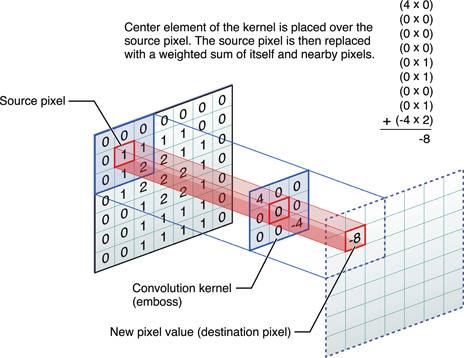
\includegraphics[scale=0.3, angle=0]{images/GvsBA.jpg}
   \end{center}
   \caption{Kernel. Two dimensions representation of the kernel action.}
  \label{fig:Kernel} 
\end{figure}



\subsection{Foward Propagation}

To perform a convolution operation, the kernel is flipped $180^{\circ}$ and slid across the input feature maps in equal and finite strides. At each location, the product between each element of the kernel and the input feature map element it overlaps is computed and the results summed up to obtain the output at that current location Eq.~(\ref{eq:convolution_tot_vox}). This procedure is repeated using different kernels to form as many output feature maps as desired Fig.~\ref{fig:features_maps}.

\subsection{Backpropagation}

For backpropagation there are two updates performed, for the weights and the deltas. Lets begin with the weight update. We are looking to compute $\partial E_{i} / \partial \omega_{uvw;l}^{(s)}$ which can be interpreted as the measurement of how the change in a single pixel $\omega_{uvw;l_{u}}^{(s)}$ in the weight kernel affects the loss function $E_{i}$. Convolution between the input feature maps of dimension $X \times Y \times Z$  and the weight kernel of dimension $I \times J \times K$ produces an output feature map of size $X \times Y \times Z$. The gradient component for the individual weights can be obtained by applying the chain rule Eq.~(\ref{eq:conv_backward_weights}).\\

%\lipsum[3-4]

\begin{equation}
  \begin{split}
    \frac{\partial E_{i}}{\partial \omega_{ijk;l_{u}}^{(s)}} =& \sum_{xyz}^{X \times Y \times Z} \frac{\partial E_{i}}{\partial a_{xyz;l_{u}}^{(s)}}\frac{\partial a_{xyz;l_{u}}^{(s)}}{\partial \omega_{ijk;l_{u}}^{(s)}}  \\
    =& \sum_{xyz}^{X \times Y \times Z} \delta_{l_{u}}^{(s)}(x,y,z) \, \sum_{s'}^{S'} z_{x'+i,y'+j,z'+k;l_{u-1}}^{(s')} \\
  \end{split}
  \label{eq:conv_backward_weights} 
\end{equation}

$\delta_{l_{u}}^{(s)}$ is the estimation of the error at the feature map $s$, at the position $(x,y,z)_{l_{u}}$ on the layer $l_{u}$. Using equation~(\ref{eq:convolution_tot_vox}) we can etimate the second part of the Eq.~(\ref{eq:conv_backward_weights}). For all activatios of the layer $l_{u}$, we have:

\begin{equation*}
  \begin{split}
    \left( \frac{\partial a_{xyz;l_{u}}}{\partial \omega_{ijk;l_{u}}} \right)^{(s)} =& \frac{\partial }{\partial \omega_{ijk;l_{u}}^{(s)}}\sum_{\sigma}\sum_{\alpha \beta \gamma} \omega_{\alpha \beta \gamma;l_{u}}^{(s)}z_{x'+\alpha,y'+\beta,z'+\gamma;l_{u-1}}^{(\sigma)}\\
    =& \sum_{\sigma}\sum_{\alpha \beta \gamma} \delta_{i \alpha} \delta_{j \beta} \delta_{k \gamma} \, z_{x'+\alpha,y'+\beta,z'+\gamma;l_{u-1}}^{(\sigma)}\\
    =& \sum_{\sigma} z_{x'+i,y'+j,z'+k;l_{u-1}}^{(\sigma)}
  \end{split}
\end{equation*}

Where $(x',y',z')$ is the center of the receptive field associated to $(x,y,z)$. In our case, the input map and the feature map have exactly the size, we should have a strict correspondance between $(x',y',z')_{l_{u-1}}$ and $(x,y,z)_{l_{u}}$. The first part of the equation, the error at the level $l_{u}$ of the feature map $s$, can be solved in the following way:

\lipsum[20-20]

\begin{strip}
\begin{equation}
  \begin{split}
    \frac{\partial E_{i}}{\partial a_{xyz;l_{u}}^{(s)}} =& \, \delta_{l_{u}}^{(s)}(x,y,z) \\ 
    =& \sum_{s''}^{S''}\sum_{x''y''z''}^{X \times Y \times Z} \frac{\partial E_{i}}{\partial a_{x''y''z'';l_{u+1}}^{(s'')}} \frac{\partial a_{x''y''z'';l_{u+1}}^{(s'')}}{\partial a_{xyz;l_{u}}^{(s)}} \\
    =& \sum_{s''}\sum_{x''y''z''} \delta_{l_{u+1}}^{(s'')}(x'',y'',z'') \frac{\partial a_{x''y''z'';l_{u+1}}^{(s'')}}{\partial a_{xyz;l_{u}}^{(s)}} \\
    =& \sum_{s''}\sum_{x''y''z''} \delta_{l_{u+1}}^{(s'')}(x'',y'',z'')  \frac{\partial }{\partial a_{xyz;l_{u}}^{(s)}} \sum_{\sigma}\sum_{\alpha \beta \gamma} \omega_{\alpha \beta \gamma;l_{u+1}}^{(s'')}z_{x''+\alpha,y''+\beta,z''+\gamma;l_{u}}^{(\sigma)} + b_{l_{u+1}}^{(s'')}\\
    =& \sum_{s''}\sum_{x''y''z''} \delta_{l_{u+1}}^{(s'')}(x'',y'',z'') \sum_{\sigma}\sum_{\alpha \beta \gamma} \omega_{ \alpha \beta \gamma;l_{u+1}}^{(s'')}  \frac{\partial }{\partial a_{xyz;l_{u}}^{(s)}} f(a_{x''+\alpha,y''+\beta,z''+\gamma;l_{u}}^{(\sigma)})\\
    =& \sum_{s''}\sum_{x''y''z''} \delta_{l_{u+1}}^{(s'')}(x'',y'',z'') \sum_{\sigma}\sum_{\alpha \beta \gamma} \omega_{ \alpha \beta \gamma;l_{u+1}}^{(s'')} \delta_{s \sigma} \delta(x-(x''+\alpha))  \delta(y-(y''+\beta))  \delta(z-(z''+\gamma))  f'(a_{x''+\alpha,y''+\beta,z''+\gamma;l_{u}}^{(\sigma)})\\
    =& f'(a_{x,y,z;l_{u}}^{(s)}) \sum_{s''}\sum_{\alpha \beta \gamma} \delta_{l_{u+1}}^{(s'')}(x-\alpha, y-\beta, z-\gamma) \, \omega_{\alpha \beta \gamma;l_{u+1}}^{(s'')}
  \end{split}
  \label{} 
\end{equation}
\end{strip}


\subsection{Up sampling}

\lipsum[21-21]

\subsection{Pooling Layer}

The function of the pooling layer is to progressively reduce the spatial size of the representation to reduce the amount of parameters and computation in the network, and hence to also control overfitting. No learning takes place on the pooling layers. Pooling units are obtained using functions like max-pooling, average pooling and even L2-norm pooling. At the pooling layer, forward propagation results in an $N \times N$ pooling block being reduced to a single value -- value of the {\it winning unit}. Backpropagation of the pooling layer then computes the error which is acquired by this single value winning unit. To keep track of the winning unit its index noted during the forward pass and used for gradient routing during backpropagation. Gradient routing is done in the following ways:

\begin{itemize}
    \item Max-pooling - the error is just assigned to where it comes from - the “winning unit” because other units in the previous layer’s pooling blocks did not contribute to it hence all the other assigned values of zero
    \item Average pooling - the error is multiplied by $1 / (N \times N)$ and assigned to the whole pooling block (all units get this same value).
\end{itemize}

%%%%%%%%%%%%%%%%%%%%%%%%%%%%%%%%%%%%%%%%%%%%%%%%%%%%%%%%%%%%%%%%%%%%%%%%%%
%%%%%%%%%%%%%%%%%%%%%%%%%%%%%%%%%%%%%%%%%%%%%%%%%%%%%%%%%%%%%%%%%%%%%%%%%%
\section{Auto-encoder}

%@inproceedings{Masci:2011:SCA:2029556.2029563,
% author = {Masci, Jonathan and Meier, Ueli and Cire\c{s}an, Dan and Schmidhuber, J\"{u}rgen},
% title = {Stacked Convolutional Auto-encoders for Hierarchical Feature Extraction},
% booktitle = {Proceedings of the 21th International Conference on Artificial Neural Networks - Volume Part I},
% series = {ICANN'11},
% year = {2011},
% isbn = {978-3-642-21734-0},
% location = {Espoo, Finland},
% pages = {52--59},
% numpages = {8},
% url = {http://dl.acm.org/citation.cfm?id=2029556.2029563},
% acmid = {2029563},
% publisher = {Springer-Verlag},
% address = {Berlin, Heidelberg},
% keywords = {auto-encoder, classification, convolutional neural network, unsupervised learning},
%} 

An auto-encoder takes an input $x \in \mathbb{R}^{d}$ and first maps it to the latent representation $\bm{h} \in \mathbb{R}^{d}$ using a deterministic function of the type $\bm{h} = f_{\theta} = \sigma(Wx + b)$ with parameters $\theta = \{W, b\}$. This "code" is then used to reconstruct the input by a reverse mapping of $\bm{y} = f_{\theta'} = \sigma( W'h + b')$ with $\theta' = \{W', b'\}$. The two parameter sets are usually constrained to be of the form $W' = W^{T}$, using the same weights for encoding the input and decoding the latent representation. The parameters are optimized, minimizing an appropriate cost function over the training set.\\

\begin{eqnarray*}
  \left(
  \begin{array}{cccc}
    \omega_{00} & \omega_{01} & \cdots & \omega_{0(n+1)} \\
    \omega_{10} & \omega_{11} & \cdots & \omega_{1(n+1)} \\
    \vdots \\
    \omega_{m0} & \omega_{m1} & \cdots & \omega_{m(n+1)} \\
  \end{array}
  \right) \left(
  \begin{array}{c}
    x_{0} \\
    x_{1} \\
    \vdots \\
    x_{n} \\
    1 \\
  \end{array}
  \right) + b = \left(
  \begin{array}{c}
    a_{0} \\
    a_{1} \\
    \vdots \\
    a_{m} 
  \end{array}
  \right)
\end{eqnarray*}

Then the decoding process $W^{T}h + b'$:

\begin{eqnarray*}
  \left(
  \begin{array}{cccc}
    \omega_{00} & \omega_{10} & \cdots & \omega_{m0} \\
    \omega_{01} & \omega_{11} & \cdots & \omega_{m1} \\
    \vdots \\
    \omega_{0(n+1)} & \omega_{1(n+1)} & \cdots & \omega_{m(n+1)} \\
  \end{array}
  \right) \left(
  \begin{array}{c}
    z_{0} \\
    z_{1} \\
    \vdots \\
    z_{m} 
  \end{array}
  \right) + b' = \left(
  \begin{array}{c}
    y_{0} \\
    y_{1} \\
    \vdots \\
    y_{n} 
  \end{array}
  \right)
\end{eqnarray*}

And we apply the back propagation epoque after epoque until $x \sim y$.

\subsection{Denoising Auto-encoder}

Without any additional constraints, conventional auto-encoders learn the identity mapping. This problem can be circumvented by using a probabilistic RBM approach, or sparse coding, or denoising auto-encoders (DAs) trying to reconstruct noisy inputs. The latter performs as well as or even better than RBMs. Training involves the reconstruction of a clean input from a partially destroyed one. Input $x$ becomes corrupted input $x'$ by adding a variable amount $v$ of noise distributed according to the characteristics of the input image. Common choices include binomial noise (switching pixels on or off) for black and white images, or uncorrelated Gaussian noise for color images. The parameter $v$ represents the percentage of permissible corruption. The auto-encoder is trained to denoise the inputs by first finding the latent representation $\bm{h} = f_{\theta} = \sigma(Wx' + b)$ frome which to reconstruct the original input $\bm{y} = f_{\theta'} = \sigma( W'h + b')$.

\subsection{Stacked Convolutional Auto-Encoders}

The trend in vision and object recognition adopted by the most successful models is to discover localized features that repeat themselves all over the input. Convolutional autoencoder differs from conventional auto-encoders as their weights are shared among all locations in the input, preserving spatial locality. The reconstruction is hence due to a linear combination of basic image patches based on the latent code. The CAE architecture is intuitively similar to the one described in the previouse section, except that the weights are shared. For a mono-channel input $x$ the latent representation of the $k$-th feature map is given by

\begin{equation*}
h^{k} = \sigma(x*W^{k} + b^{k})
\end{equation*}

The reconstruction is obtained using

\begin{equation*}
y = \sigma \left(\sum_{k \in H} h^{k}*\tilde{W}^{k} + c \right)
\end{equation*}

where again there is one bias $c$ per input channel. $H$ identifies the group of latent feature maps; $\tilde{W}$ identifies the flip operation over both dimensions of the weights. The cost function to minimize is the mean squared error (MSE):

\begin{equation*}
E= \frac{1}{2n} \sum_{i=1}^{n} ( x_{i} - y_{i})^{2}
\end{equation*}

\subsubsection{Mathematical description of the backpropagation}

An auto-encoder takes an input $z_{l_{u-1}}^{(s)} \in \mathbb{R}^{d}$ and first maps it to the latent representation $a_{l_{u}^{(\sigma)}} \in \mathbb{R}^{d}$ using a deterministic function of the type $z_{x,l_{u}}^{(\sigma)} = f_{\theta}(\sum_{s,\epsilon} \omega_{\epsilon,l_{u}}^{(\sigma)}z_{x+\epsilon,l_{u-1}}^{(s)} + b_{l_{u}}^{(\sigma)})$ with parameters $\theta = \{\omega_{l_{u}}, b_{l_{u}}^{(\sigma)}\}$. This "code" is then used to reconstruct the input by a reverse mapping of $z_{x,l_{u+1}}^{(s)} = f_{\theta'}(\sum_{\sigma,\epsilon} \omega_{\epsilon,l_{u}}^{(\sigma)}z_{x-\epsilon,l_{u}}^{(\sigma)} + b_{l_{u+1}}^{(s)})$ with $\theta_{l_{u+1}} = \{W', b_{l_{u+1}}^{(s)}\}$. The two parameter sets are usually constrained to be of the form $W' = W_{l_{u}}^{T}$, using the same weights for encoding the input and decoding the latent representation. The parameters are optimized, minimizing an appropriate cost function over the training set. In all the equations $(s)$ represents the number of inputs and $(\sigma)$ the number of feature maps created in the process. In the auto-encoder, the number of inputs and final outputs can match. In other uses, {\it e.g.} the segmentation, the number of input can be the different acquisition types and the number of outputs can different segmentations.\\
The encoding level is similar to a convolutional layer: in a kernel window of $\epsilon$ elements, activations $a_{x,l_{u}}^{\mu}$ at the position $x$ in the layer $l_{u}$ 

\begin{eqnarray*}
  \left(
  \begin{array}{cccc}
    \omega_{0}^{(1)} & \omega_{1}^{(1)} & \cdots & \omega_{(\nu)}^{(1)} \\
    \omega_{0}^{(2)} & \omega_{1}^{(2)} & \cdots & \omega_{(\nu)}^{(2)} \\
    \vdots \\
    \omega_{0}^{(\sigma)} & \omega_{1}^{(\sigma)} & \cdots & \omega_{(\nu)}^{(\sigma)} \\
  \end{array}
  \right)_{l_{u}} \left(
  \begin{array}{c}
    z_{0} \\
    z_{1} \\
    \vdots \\
    z_{\nu-1} \\
    1 \\
  \end{array}
  \right)_{l_{u-1}}^{(1,2,\cdots,s)} + b_{l_{u}}^{(\sigma)}= \left(
  \begin{array}{c}
    a^{(1)} \\
    a^{(2)} \\
    \vdots \\
    a^{(\sigma)} 
  \end{array}
  \right)_{x,l_{u}}
\end{eqnarray*}

Wich can be written: $z_{x,l_{u}}^{(\sigma)} = f(a_{x,l_{u}}^{(\sigma)})$ where $a_{x,l_{u}}^{(\sigma)} = \sum_{\epsilon,s} \omega_{\epsilon,l_{u}}^{(\sigma)}z_{x+\epsilon,l_{u-1}}^{(s)} + b_{l_{u}}^{(\sigma)}$. In a similar way, as the auto-encoder, we can use the same set of weights for the convolutional auto-encoder, then we can write


\begin{strip}
  \begin{eqnarray*}
      \left(
      \begin{array}{cccc}
        \omega_{0}^{(1)} & \omega_{0}^{(2)} & \cdots & \omega_{0}^{(\sigma)} \\
        \omega_{1}^{(1)} & \omega_{1}^{(2)} & \cdots & \omega_{1}^{(\sigma)} \\
        \vdots \\
        \omega_{\nu-1}^{(1)} & \omega_{\nu-1}^{(2)} & \cdots & \omega_{\nu-1}^{(\sigma)} \\
      \end{array}
      \right) \left(
      \begin{array}{c}
        z_{0}^{(1)} \\
        z_{0}^{(2)} \\
        \vdots \\
        z_{0}^{(\sigma)} \\
      \end{array}
      \right) + \left. 
      \begin{array}{c}
        z_{1}^{(1)} \\
        z_{1}^{(2)} \\
        \vdots \\
        z_{1}^{(\sigma)} \\
      \end{array}
      \right) + \cdots + \left. 
      \begin{array}{c}
        z_{\nu-1}^{(1)} \\
        z_{\nu-1}^{(2)} \\
        \vdots \\
        z_{\nu-1}^{(\sigma)} \\
      \end{array}
      \right)_{x,l_{u}} + b_{l_{u+1}}^{(s)};~and~f_{\theta}\left(\sum_{\sigma} z_{l_{u}}^{(\sigma)}*\tilde{W}^{(\sigma)} + b_{l_{u+1}}^{(s)} \right) = y_{x,l_{u+1}}^{(s)}
  \end{eqnarray*}
\end{strip}

This can be written in a more compact way, $z_{x,l_{u+1}}^{(\nu)} = f(a_{x,l_{u+1}}^{(\nu)})$ where $(\nu)$ can be equal to $(s)$ in the auto-encoder algorithm. And $a_{x,l_{u+1}}^{(\nu)} = \sum_{\epsilon,\sigma} \omega_{\epsilon,l_{u}}^{(\sigma)}z_{x+\epsilon,l_{u}}^{(\sigma)} + b_{l_{u+1}}^{(\nu)}$. \\
We have two levels of the auto-encoder sharing the same weights. We can use the backpropagation through the two levels. In this example, the loss function is the sum of squares $E_{i} = \sum_{s} (z_{l_{u-1}}^{(s)} - z_{l_{u+1}}^{(s)})^{2}$. As usual, we start with:

\begin{eqnarray}
  \frac{\partial E_{i}}{\partial \omega_{\epsilon',l_{u}}^{(\sigma')}} & = & \sum_{\nu,x} \frac{\partial E_{i}}{\partial a_{x,l_{u+1}}^{(\nu)}} \frac{a_{x,l_{u+1}}^{(\nu)}}{\partial \omega_{\epsilon',l_{u}}^{(\sigma')}} + \sum_{\sigma,x} \frac{\partial E_{i}}{\partial a_{x,l_{u}}^{(\sigma)}} \frac{a_{x,l_{u}}^{(\sigma)}}{\partial \omega_{\epsilon',l_{u}}^{(\sigma')}} \\
 & = & \sum_{\nu,x} \delta_{l_{u+1}}^{(\nu)}(x) \frac{a_{x,l_{u+1}}^{(\nu)}}{\partial \omega_{\epsilon',l_{u}}^{(\sigma')}} + \sum_{\sigma,x} \delta_{l_{u}}^{(\sigma)}(x) \frac{a_{x,l_{u}}^{(\sigma)}}{\partial \omega_{\epsilon',l_{u}}^{(\sigma')}} \\
 & = & \sum_{\nu} \delta_{l_{u+1}}^{(\nu)} \underset{\epsilon'}{*} z_{l_{u}}^{(\sigma')}  + \sum_{s} \delta_{l_{u}}^{(\sigma')} \underset{\epsilon'}{*} z_{l_{u-1}}^{(s)}  \\
\end{eqnarray}
\label{equa:AE_1}

Where $\underset{\epsilon'}{*}$ represents the center $\epsilon'$ of the window convolved across the entire image. The last equation can be found using the following evaluation:

\begin{eqnarray*}
  \left \lbrace
  \begin{array}{rcl}
    \frac{a_{x,l_{u}}^{(\sigma)}}{\partial \omega_{\epsilon',l_{u}}^{(\sigma')}} & = & \sum_{s,\epsilon} \delta_{\epsilon' \epsilon} \delta_{\sigma' \sigma} z_{x+\epsilon,l_{u-1}}^{(s)} = \sum_{s} \delta_{\sigma' \sigma} z_{x+\epsilon',l_{u-1}}^{(s)}\\
    \delta_{l_{u}}^{(\sigma)}(x) & = & \sum_{\nu,x'} \frac{\partial E_{i}}{\partial a_{x',l_{u+1}}^{(\nu)}}\frac{\partial a_{x',l_{u+1}}^{(\nu)}}{\partial a_{x,l_{u}}^{(\sigma)}} = \sum_{\nu,x'} \delta_{l_{u+1}}^{(\nu)}(x')\frac{\partial a_{x',l_{u+1}}^{(\nu)}}{\partial a_{x,l_{u}}^{(\sigma)}} \\
    & = & \sum_{\nu,x'} \delta_{l_{u+1}}^{(\nu)}(x') \sum_{\sigma'',\epsilon} \omega_{\epsilon,l_{u}}^{(\sigma'')} (f')_{x'+\epsilon,l_{u}}^{(\sigma'')} \\
    & \times & \delta_{\sigma'' \sigma} \delta(x - (x'-\epsilon)) \\
    & = & \sum_{\nu,\epsilon} \delta_{l_{u+1}}^{(\nu)}(x-\epsilon) \omega_{\epsilon,l_{u}}^{(\sigma)} (f')_{x,l_{u}}^{(\sigma)}
  \end{array}
  \right .
\end{eqnarray*}

The second level can be evaluated:

\begin{eqnarray*}
  \left \lbrace
  \begin{array}{rcl}
    \frac{a_{x,l_{u+1}}^{(\nu)}}{\partial \omega_{\epsilon',l_{u}}^{(\sigma')}} & = & \sum_{\sigma,\epsilon} \delta_{\epsilon' \epsilon} \delta_{\sigma' \sigma} z_{x+\epsilon,l_{u}}^{(\sigma)} = z_{x+\epsilon',l_{u}}^{(\sigma')} \\
    \delta_{l_{u+1}}^{(\nu)}(x) & = & \left( z_{l_{u-1}}^{(\nu)} - z_{l_{u+1}}^{(\nu)} \right) f'(a_{x,l_{u+1}}^{(\nu)})
  \end{array}
  \right .
\end{eqnarray*}
  


%%%%%%%%%%%%%%%%%%%%%%%%%%%%%%%%%%%%%%%%%%%%%%%%%%%%%%%%%%%%%%%%%%%%%%%%%%
%%%%%%%%%%%%%%%%%%%%%%%%%%%%%%%%%%%%%%%%%%%%%%%%%%%%%%%%%%%%%%%%%%%%%%%%%%
\section{Densely connected neural network}

Dense neural networks are caracterized by a full connection of a neurons of one layer with all neurons plus the bias from the previouse layer Fig.~\ref{fig:Densely_connected_neural_network}. Table~\ref{Layers_activations} presents the activation function for each layer. Each neuron, or activation, of a layer is the result of a perceptron, built from all the nerons of the previous layer and the bias, and filtered by an activation function. 

\subsection{Description and notation}

In this document, the convention is $l = l_{0}$ for the input layer: $z_{l_{0} = 1} = x_{1}$, $z_{l_{0} = 2} = x_{2}$, \dots We will reserve the index 0 for the bias: $z_{l_{0} = 0} = x_{0} = b_{0}$ the bias on the input level. The last level is the output level: $l = l_{k}$, $z_{l_{k}} = y_{k}$. The output level does not have a bias node.

\begin{table}[]
\centering
\caption{Neuron activation for each layers.}
\label{Layers_activations}
\begin{tabular}{llllll}
  \hline
 $\{ z_{l_{0}}\}_{l_{0} = 0}^{L_{0}}$&  $\{ z_{l_{1}}\}_{l_{1} = 0}^{L_{1}}$ &  $\cdots$ & $\{ z_{l_{k-1}}\}_{l_{k-1} = 0}^{L_{k-1}}$ &  $\{ z_{l_{k}}\}_{l_{k} = 0}^{L_{k}-1}$ &  \\ 
  \hline
\end{tabular}
\end{table}

\begin{figure}[htbp]
   \begin{center}
      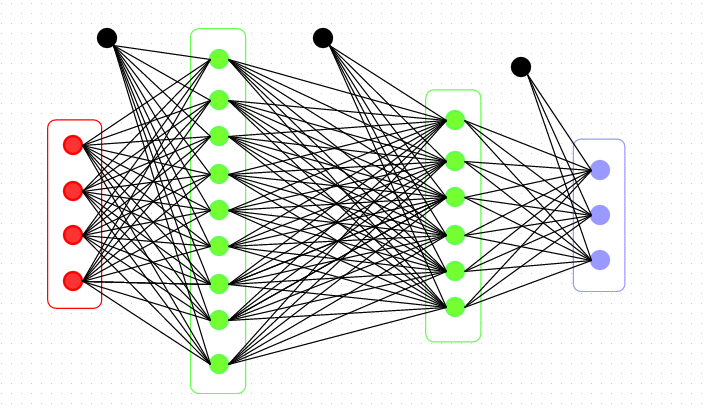
\includegraphics[scale=0.3, angle=0]{images/densely_connected_nn.png}
   \end{center}
   \caption{Densely connected neural network. The red dots represnet the input, the green dots represent the hidden layers, the blue dots represent the output layer. the black dots are the bias. The output layer is the only layer without a bias weight.}
  \label{fig:Densely_connected_neural_network} 
\end{figure}

Each neuron is an activated function, $f$, of a linear combinaison of the neurons from the previous layer. Function $g$ is the activation function for the output layer.

\begin{itemize}
    \item $l = l_{0}$ we are at the level of the inputs
    \item $l = l_{1}$ $a_{l_{1}} = \sum_{l'_{0} = 0}^{L_{0}} \omega_{l_{1}l'_{0}} z_{l'_{0}}$. And $z_{l_{1}} = f(a_{l_{1}})$ \\
     $\vdots$
    \item $l = l_{k-1}$ $a_{l_{k-1}} = \sum_{l'_{k-2} = 0}^{L_{k-2}} \omega_{l_{k-1}l'_{k-2}} z_{l'_{k-2}}$. And $z_{l_{k-1}} = f(a_{l_{k-1}})$ \\ 
    \item $l = l_{k}$ $a_{l_{k}} = \sum_{l'_{k-1} = 0}^{L_{k-1}} \omega_{l_{k}l'_{k-1}} z_{l'_{k-1}}$. And $z_{l_{k}} = g(a_{l_{k}})$
\end{itemize}

At each layer, activations can be represented as a vector:

\begin{eqnarray*}
  \left(
  \begin{array}{c}
    a_{l_{1} = 0} \\
    a_{l_{1} = 1} \\
    \vdots \\
    a_{L_{1} - 1}
  \end{array}
  \right) = \left(
  \begin{array}{cccc}
    \omega_{00} & \omega_{01} & \cdots & \omega_{0L_{0}} \\
    \omega_{10} & \omega_{11} & \cdots & \omega_{1L_{0}} \\
    \vdots     &            & \cdots & \vdots \\
    \omega_{(L_{1}-1)0} & \omega_{(L_{1}-1)1} & \cdots & \omega_{(L_{1}-1)L_{0}} \\
  \end{array}
  \right)  \left(
  \begin{array}{c}
    z_{l_{0} = 0} \\
    z_{l_{0} = 1} \\
    \vdots \\
    z_{L_{0} - 1} \\
    1
  \end{array}
  \right)
\end{eqnarray*}

Which can be writen in a compact manner: $\bm{a}^{(l_{1})} = \Omega_{10}\bm{z}^{(l_{0})}$. The 1 at the end of the $\bm{z}$ vector represents the bias terme. Following he same writing, the forward algorithm can be written: $\bm{a} = \Omega\bm{z}$, where $\Omega$ is a block-diagonal matrix:

\begin{eqnarray*}
  \Omega = \left(
  \begin{array}{cccc}
    \Omega_{10} &            & 0      &  \\
               & \Omega_{21} &        &  \\
               &            & \ddots &  \\
               & 0          &        & \Omega_{k(k-1)} \\
  \end{array}
  \right)
\end{eqnarray*}

  There are several choises for the activation function and we will try to provide the possibility of using several of them. However, the first developpments will be done with the hyperbolic tangent for the activation of the inside layers neurons: $f = \tanh$ and $f' = (1 - \tanh^{2})$. The last layer, the output layer, will be calculated with a soft maximum: $g(z_{l_{k}}) = e^{a_{l_{k}}} / \mathcal{Z}$, where the partition function $\mathcal{Z} = \sum_{l_{k} = 1}^{L_{k}} e^{z_{l_{k}}}$, and $g' = g(1 - g)$.
  
\subsection{Forward propagation}

The forward propagation is straight forward. For a solution, $y_{k} = z_{l_{k}} = g(a_{l_{k}})$ where
$$
a_{l_{k}} = \omega_{l_{k}}^{T} z^{(k-1)} = \omega_{l_{k}}^{T} f(\omega_{l_{k-1}}^{T} z^{(k-2)}) = \omega_{l_{k}}^{T} f(\omega_{l_{k-1}}^{T} f(\omega_{l_{k-2}}^{T} z^{(k-3)})) = \dots
$$

\subsubsection{Algorithm}

The Table~\ref{weights_in_mem} gives the distribution of the weights in a dense neural network. These weights can be represented in one long array in the hardware memory. The first layer $l = l_{1}$, after the inputs, has $(L_{0}+1)\times(L_{1})$ weights. The layer after has $(L_{1}+1)\times(L_{2})$ weights, so forth till the last layer having $(L_{k-1}+1)\times(L_{k})$.


\begin{table}[]
\centering
\caption{Representation in a one dimension array of the all the weights.}
\label{weights_in_mem}
\begin{tabular}{|c|c|c|c|c|c|c|c|}
\hline
\multicolumn{4}{|c|}{$l_{1}$} & $\hdots$ & \multicolumn{3}{c|}{$l_{k}$} \\ \hline
$\omega_{l_{1}=0l_{0}=0}$   &   $\omega_{01}$   & $\hdots$  &  $\omega_{(L_{1}-1)L_{0}}$   & $\hdots$ &    $\omega_{l_{k}=0l_{k-1}=0}$    & $\hdots$  &   $\omega_{(L_{k}-1)L_{k-1}}$ \\ \hline
\end{tabular}
\end{table}

%%%%%%%%%%%%%%%%%%%%%%%%%%%%%%%%%%%%%%%%%%%%%%%%%%%%%%%%%%%%%%%%%%%%%%%%%%
%%%%%%%%%%%%%%%%%%%%%%%%%%%%%%%%%%%%%%%%%%%%%%%%%%%%%%%%%%%%%%%%%%%%%%%%%%
\subsection{Backward propagation}

To solve the problem of the backward propagation, we have three options. The first option is to estimate the error for the full training set, which is heavy for the algorithm. The second option is the gradient descent in its stochastic version: each iteration will use a new intput, instead of estimating the cost function with the entire input population. The third option is a mid-point between the two first options: the error is estimated with a sub set of the full training set.
Taking the cross-enropy cost function, eq.~(\ref{cross_entropy}), in the case of classification. The gradient descent method used to find the minimum of the cost function is written:

\begin{equation}
  \bm{\omega}^{e+1} = \bm{\omega}^{e} - \eta \bm{\nabla} E
  \label{gradient_descent}
\end{equation}

Where $\bm{\omega}$ represents the vector of weights, $e$ represents the {\it epoque} (iteration), and $\eta$ represents the learning rate. 


%%%%%%%%%%%%%%%%%%%%%%%%%%%%%%%%%%%%%%%%%%%%%%%%%%%%%%%%%%%%%%%%%%%%%%%%%%
\subsubsection{Algorithm}

The backward propagation for each layer, except the last layer, is a recursive estimtion of the deeper layer. The gradient Eq.~(\ref{gradient_descent}) at a particular weight is, using the error Eq.~(\ref{cost_function_error}),

\begin{equation*}
  \frac{\partial E_{i}}{\partial \omega_{l_{u}l_{v}}} = \frac{\partial E_{i}}{\partial a_{l_{u}}} \frac{\partial a_{l_{u}}}{\partial \omega_{l_{u}l_{v}}} = \delta_{l_{u}}\frac{\partial a_{l_{u}}}{\partial \omega_{l_{u}l_{v}}} 
\end{equation*}


\paragraph{$\bm{l = l_{k}}$}{ Using the results from the section~\ref{Cross_entropy_cost_function_sec}:

  \begin{equation*}
    \begin{split}
      \frac{\partial E_{i}}{\partial \omega_{l_{k}l_{k-1}}} = &  \frac{\partial E_{i}}{\partial a_{l_{k}}} \frac{\partial a_{l_{k}}}{\partial \omega_{l_{k}l_{k-1}}}  \\
              = &  (z_{l_{k}} - t_{l_{k}})z_{l_{k-1}} \\
    \end{split}
  \end{equation*}

}

\paragraph{$\bm{l = l_{u}}$}{We write the relation between the level $l_{u}$ and the layer immediatly after using the chain rules of partial derivative:

  \begin{equation*}
    \begin{split}
      \frac{\partial E_{i}}{\partial \omega_{l_{u}l_{u-1}}} = &  \frac{\partial E_{i}}{\partial a_{l_{u}}} \frac{\partial a_{l_{u}}}{\partial \omega_{l_{u}l_{u-1}}} = \delta_{l_{u}} \frac{\partial a_{l_{u}}}{\partial \omega_{l_{u}l_{u-1}}}  \\
              = & \sum_{l'_{u+1}}\frac{\partial E_{i}}{\partial a_{l'_{u+1}}} \frac{\partial a_{l'_{u+1}}}{\partial a_{l_{u}}} \frac{\partial a_{l_{u}}}{\partial \omega_{l_{u}l_{u-1}}}   \\
              = & \sum_{l'_{u+1}} \delta_{l'_{u+1}} \frac{\partial a_{l'_{u+1}}}{\partial a_{l_{u}}} z_{l_{u-1}}   \\
              = & \sum_{l'_{u+1}} \delta_{l'_{u+1}} \sum_{l'_{u}} \omega_{l'_{u+1}l'_{u}} f'(a_{l'_{u}}) \delta_{l'_{u}l_{u}} z_{l_{u-1}}   \\
              = & \sum_{l'_{u+1}} \delta_{l'_{u+1}} \omega_{l'_{u+1}l_{u}} f'(a_{l_{u}}) z_{l_{u-1}}   \\
    \end{split}
\end{equation*}

}


%%%%%%%%%%%%%%%%%%%%%%%%%%%%%%%%%%%%%%%%%%%%%%%%%%%%%%%%%%%%%%%%%%%%%%%%%%
%%%%%%%%%%%%%%%%%%%%%%%%%%%%%%%%%%%%%%%%%%%%%%%%%%%%%%%%%%%%%%%%%%%%%%%%%%
\section{Verification and Validation}
\lipsum[20-20]

%%%%%%%%%%%%%%%%%%%%%%%%%%%%%%%%%%%%%%%%%%%%%%%%%%%%%%%%%%%%%%%%%%%%%%%%%%
\subsection{Vanishing gradient}

The vanishing gradient problem affects many-layered feedforward networks that used backpropagation and also recurrent neural networks (RNNs). As errors propagate from layer to layer, they shrink exponentially with the number of layers, impeding the tuning of neuron weights that is based on those errors, particularly affecting deep networks. Hinton et al. (2006) proposed learning a high-level representation using successive layers of binary or real-valued latent variables with a restricted Boltzmann machine[21] to model each layer. Once sufficiently many layers have been learned, the deep architecture may be used as a generative model by reproducing the data when sampling down the model (an "ancestral pass") from the top level feature activations.\\
\lipsum[19-19]


%%%%%%%%%%%%%%%%%%%%%%%%%%%%%%%%%%%%%%%%%%%%%%%%%%%%%%%%%%%%%%%%%%%%%%%%%%
\subsection{Early stoping}
\lipsum[21-21]
%%%%%%%%%%%%%%%%%%%%%%%%%%%%%%%%%%%%%%%%%%%%%%%%%%%%%%%%%%%%%%%%%%%%%%%%%%
\subsection{Drop out}
\lipsum[22-22]


%%%%%%%%%%%%%%%%%%%%%%%%%%%%%%%%%%%%%%%%%%%%%%%%%%%%%%%%%%%%%%%%%%%%%%%%%%
%%%%%%%%%%%%%%%%%%%%%%%%%%%%%%%%%%%%%%%%%%%%%%%%%%%%%%%%%%%%%%%%%%%%%%%%%%
\section{Monte-Rosa}

\lipsum[30-33]

Eventually with a small enough feature map, the contents are squashed into a one dimension vector and fed into a fully-connected MLP for processing. The last layer of this fully-connected MLP seen as the output, is a loss layer which is used to specify how the network training penalizes the deviation between the predicted and true labels.


%%%%%%%%%%%%%%%%%%%%%%%%%%%%%%%%%%%%%%%%%%%%%%%%%%%%%%%%%%%%%%%%%%%%%%%%%%
%%%%%%%%%%%%%%%%%%%%%%%%%%%%%%%%%%%%%%%%%%%%%%%%%%%%%%%%%%%%%%%%%%%%%%%%%%
\section{Mont-Blanc}

\lipsum[40-43]

%%%%%%%%%%%%%%%%%%%%%%%%%%%%%%%%%%%%%%%%%%%%%%%%%%%%%%%%%%%%%%%%%%%%%%%%%%
%%%%%%%%%%%%%%%%%%%%%%%%%%%%%%%%%%%%%%%%%%%%%%%%%%%%%%%%%%%%%%%%%%%%%%%%%%
\section{Conclusion}

\lipsum[6-10]

\section*{References}
%% References with bibTeX database:
\bibliographystyle{Bibliography/elsarticle-num}

\bibliography{Bibliography/sample}


\end{document}
